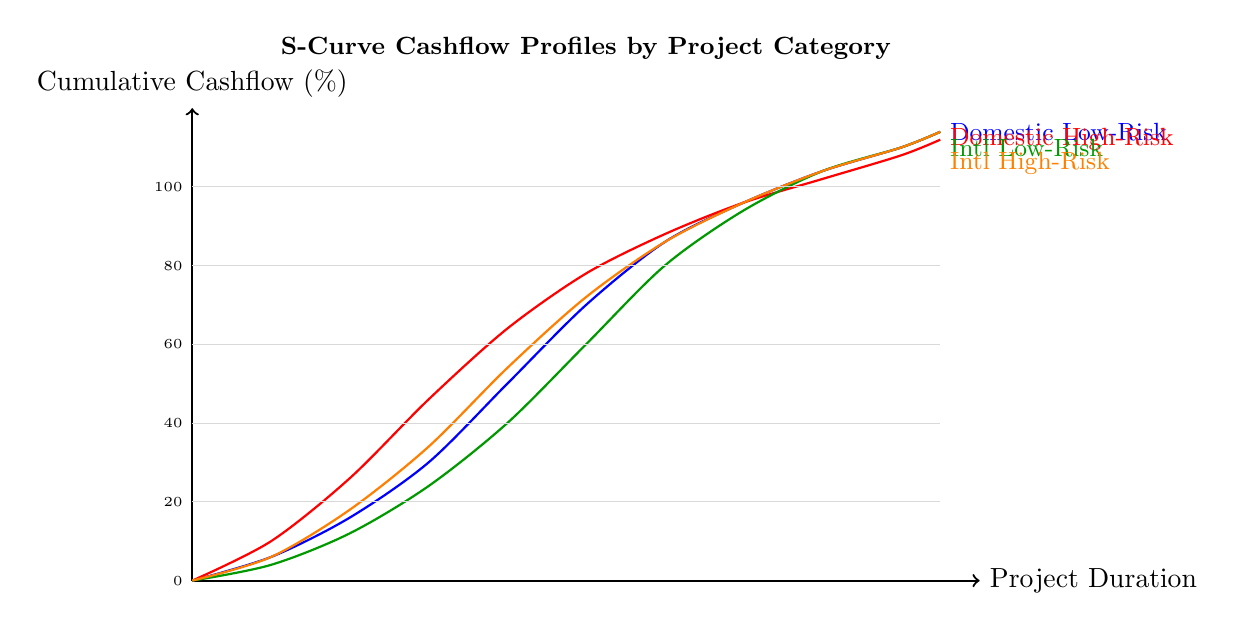
\begin{tikzpicture}[scale=1.0]
    % Axes
    \draw[thick, ->] (0,0) -- (10,0) node[right] {Project Duration};
    \draw[thick, ->] (0,0) -- (0,6) node[above] {Cumulative Cashflow (\%)};
    
    % S-curves for different categories
    % Domestic Low-Risk (symmetric)
    \draw[thick, blue, smooth] plot coordinates {
        (0,0) (1,0.3) (2,0.8) (3,1.5) (4,2.5) (5,3.5) (6,4.3) (7,4.8) (8,5.2) (9,5.5) (9.5,5.7)
    };
    \node[right, blue, font=\small] at (9.5,5.7) {Domestic Low-Risk};
    
    % Domestic High-Risk (early peak)
    \draw[thick, red, smooth] plot coordinates {
        (0,0) (1,0.5) (2,1.3) (3,2.3) (4,3.2) (5,3.9) (6,4.4) (7,4.8) (8,5.1) (9,5.4) (9.5,5.6)
    };
    \node[right, red, font=\small] at (9.5,5.6) {Domestic High-Risk};
    
    % International Low-Risk (late peak)
    \draw[thick, green!60!black, smooth] plot coordinates {
        (0,0) (1,0.2) (2,0.6) (3,1.2) (4,2.0) (5,3.0) (6,4.0) (7,4.7) (8,5.2) (9,5.5) (9.5,5.7)
    };
    \node[right, green!60!black, font=\small] at (9.5,5.5) {Intl Low-Risk};
    
    % International High-Risk (mid peak, heavy tail)
    \draw[thick, orange, smooth] plot coordinates {
        (0,0) (1,0.3) (2,0.9) (3,1.7) (4,2.7) (5,3.6) (6,4.3) (7,4.8) (8,5.2) (9,5.5) (9.5,5.7)
    };
    \node[right, orange, font=\small] at (9.5,5.3) {Intl High-Risk};
    
    % Grid
    \foreach \y in {1,2,3,4,5} {
        \draw[gray!30] (0,\y) -- (9.5,\y);
    }
    
    % Y-axis labels
    \foreach \y in {0,20,40,60,80,100} {
        \node[left, font=\tiny] at (0,\y/20) {\y};
    }
    
    % Title
    \node[above, font=\small\bfseries] at (5,6.5) {S-Curve Cashflow Profiles by Project Category};
\end{tikzpicture}
